
\def\MIN{
  \question[1]
  Simplificar as expressões Booleanas:
  
  \begin{parts}
    \part
    $\!{ \!{{(s\+\!t)}} \+ \!{(s\+\!u)} \+ v}$

    \begin{solution}
      $(s + \!t)(s + \!u) \!v$
    \end{solution}

    \part
    $\!xyz \+ x\!yz \+ xy\!z \+ xyz$
    \begin{solution}
      $yz+xz+xy$
    \end{solution}

    \part
    $\!x(x\+y) \+ (y\+x)(x\+\!y)$
    \begin{solution}
      $x+y$
    \end{solution}


    \part
    $\!{ \!{x\+yz}\ {\!{x\!y}} }$
    \begin{solution}
      $x+yz$
    \end{solution}

  \end{parts}
}

\def\theorems{\footnotesize
\hfil {\bf Teoremas Booleanos}
\begin{tabbing}
  \noindent \=T1. Elemento nulo: \hspace{1cm}\= $x+1=1$\hspace{3cm}\= $x.0=0$\\
  \> T2. Idempotência:\> $x+x=x$ \>$ x.x=x$ \\
  \> T3. Absorção: \>$x+x.y=x $ \>$ x.(x+y) = x$ \\
  \> T4. Adsorção: \>$(\!x+y).x=x.y $ \>$ x+\!x.y = x+y$ \\
  \> T5. Associatividade: \> $(x+y)+z=x+(y+z)$ \> $(x.y).z = x.(y.z)$\\
  \> T6. De Morgan: \> $\!{x+y} = \!x.\!y$ \> $\!{x.y} = \!x + \!y$ \\
\end{tabbing}

}

\def\ALSdecoder{ \question[1] Determine os níveis de cada saída do
  decodificador mostrado na Figura~\ref{fig:alsdecoder} para as
  seguintes condições de entrada:

\begin{parts}
\part
Todas as entradas em nível baixo;
\part
Todas as entradas em nível baixo, exceto $e_3=1$;
\part
Todas as entradas em nível alto, exceto $\!e_1=\!e_2=0$;
\part
Todas as entradas em nível alto.
\end{parts}

  \begin{figure}[ht]
    \centering
    \begin{tikzpicture}
  \def\w{2cm}\footnotesize
  \def\h{\w/2}
  \def\r{2.5pt}
  \node[rectangle, minimum height=\h, minimum width=2.5*\w, draw] (DECODER) {decodificador 74ALS138};
  \foreach \X/\x in {2/0,1/.5,0/1}{
    \path[draw] (DECODER.north west)+(\x,0) -- +(\x, \h) node[above] {$x_\X$};
  }
  \foreach \f/\x in {7/0,6/.5,5/1,4/1.5,3/2,2/2.5,1/3,0/3.5}{
    \draw (DECODER.south west)[yshift=-\r,xshift=\x cm] circle (\r) node (INV\f) {};
    \path[draw] (INV\f) -- +(0, -\h) node[below] {$\overline{f_\f}$};
  }
  \node[minimum height=\h,anchor=east,draw,and gate US,rotate=-90] (AND) at (DECODER.north east)[yshift=-\h] {};
  \foreach \p/\e in {south west/1, mid west/2}{
    \draw[]  (AND.\p)[yshift=\r] circle (\r) node (AINV\p) {};
    \path[draw] (AND.\p)+(0,2*\r) -- +(0,\h/2) node[above] {$\overline{e_\e}$};
  }
  \path[draw] (AND.north west) -- +(0,\h/2) node[above] {$e_3$};
\end{tikzpicture}


    \caption{Decodificador 74ALS138.}
    \label{fig:alsdecoder}
  \end{figure}

  \begin{solution}
    \begin{enumerate}[a)]
    \item $f_0=f_1=f_2=f_3=f_4=f_5=f_6=f_7=1$
      \item $f_0=0$
      \item $f_7=0$
      \item $f_0=f_1=f_2=f_3=f_4=f_5=f_6=f_7=1$
    \end{enumerate}
  \end{solution}

\question[1]
Para que condições de entrada produzirão as seguintes saídas no
decodificador mostrado na Figura~\ref{fig:alsdecoder}?

\begin{parts}
  \part
  Nível baixo em $f_6$;
  \part
  Nível baixo em $f_3$;
  \part
  Nìvel baixo em $f_5$;
  \part
  Nível baixo em $f_0$ e $f_7$, simultaneamente.
\end{parts}


  \begin{solution}
    \begin{enumerate}[a)]
    \item $f(x_2,x_1,x_0,e_1,e_2,e_3)=f(1,1,0,0,0,1)$
      \item $f(x_2,x_1,x_0,e_1,e_2,e_3)=f(0,1,1,0,0,1)$
      \item $f(x_2,x_1,x_0,e_1,e_2,e_3)=f(1,0,1,0,0,1)$
      \item $f(x_2,x_1,x_0,e_1,e_2,e_3)=\emptyset$, não há condições para esta saída
    \end{enumerate}
  \end{solution}
}

\def\MUX74HC151{

  \question[2]~O circuito da Figura~\ref{fig:mux74hc151} mostra como
  um mux 74HC151 de 8 entradas pode ser usado para gerar uma função de
  4 variáveis lógicas. Três das variáveis lógicas, $x_0, x_1, x_2$ são
  conectadas na entrada de seleção. A quarta variável, $x_3$, e seu
  inverso, $\overline{x_3}$, são conectadas em entradas de dados
  selecionadas do mux, conforme requer a função lógica desejada. As
  outras entradas de dados são conectadas em nível baixo ou alto,
  conforme requer a função lógica.

\begin{parts}
  \part
  Construa a tabela-verdade mostrando a saída $f(x_0,x_1,x_2,x_3)$
  para as 16 combinações possíveis das variáveis de entrada.
  \part
  Escreva a função $f(x_0,x_1,x_2,x_3)$ na forma normal disjuntiva e
  simplifique-a.

\end{parts}

\begin{figure}[ht]
\centering
\begin{tikzpicture}
  \def\w{2cm}\footnotesize
  \def\h{\w/2}
  \def\r{2.5pt}
  \node[rectangle, minimum height=2*\h, minimum width=2.5*\w, draw] (MUX) {mux 74HC151};
  \foreach \Y/\y in {2/-.2,1/.3,0/.8}{
    \path[draw] (MUX.west)+(0,-\y) node[right] {$s_\Y$} -- +(-\w, -\y) node[above] {$x_\Y$};
  }
  \foreach \i/\v/\x in {7/0/0.5,6/0/1,5/0/1.5,4/\overline{x_3}/2,3/0/2.5,2/1/3,1/x_3/3.5,0/0/4}{
    \path[draw] (MUX.north east)+(-\x,0) node[below] (I\i) {$i_\i$} -- +(-\x, \h) node[above] {$\v$};
  }
  \node[fill=white,anchor=east,draw,not gate US,rotate=-90] (AND) at (I4.north)[] {};

  \path[draw] (MUX.south) -- +(0,-1.5*\h) 
  node[below] (F) {$f(i_0,i_1,i_2,i_3,i_4,i_5,i_6,i_7,s_0,s_1,s_2) = $};
  \node[text width=.3\textwidth] [right of=F,xshift=4.25cm] 
  {$\!s_0\,\!s_1\,\!s_2i_0 + 
    \!s_0\,\!s_1s_2i_1 + 
    \!s_0s_1\,\!s_2i_2 +
    \!s_0\,s_1s_2i_3 +
    s_0\!s_1\,\!s_2i_4 + 
    s_0\!s_1s_2i_5 + 
    s_0s_1\!s_2i_6 + 
    s_0s_1s_2i_7$ };
 
\end{tikzpicture}

\caption{Implementação de função lógica usando o multiplexador modelo
  74HC151.}
\label{fig:mux74hc151}
\end{figure}

\begin{solution}
  \begin{enumerate}[a)]
  \item $f(x_0,x_1,x_2,x_3)=\!x_0\,\!x_1x_2x_3 + \!x_0x_1\!x_2 + x_0\!x_1\!x_2\!x_3$\\
    \begin{center}
      \begin{tabular}[ht]{cccc|c}
        $x_0$& $x_1$ & $x_2$ & $x_3$ & $f(x_0,x_1,x_2,x_3)$\\\hline
        0 & 0 & 0 & 0 & 0\\
        0 & 0 & 0 & 1 & 0\\
        0 & 0 & 1 & 0 & 0\\
        0 & 0 & 1 & 1 & 1\\
        0 & 1 & 0 & 0 & 1\\
        0 & 1 & 0 & 1 & 1\\
        0 & 1 & 1 & 0 & 0\\
        0 & 1 & 1 & 1 & 0\\
        1 & 0 & 0 & 0 & 1\\
        1 & 0 & 0 & 1 & 0\\
        1 & 0 & 1 & 0 & 0\\
        1 & 0 & 1 & 1 & 0\\
        1 & 1 & 0 & 0 & 0\\
        1 & 1 & 0 & 1 & 0\\
        1 & 1 & 1 & 0 & 0\\
        1 & 1 & 1 & 1 & 0\\
    \end{tabular}
  \end{center}
\item $f_{FND}(x_0,x_1,x_2,x_3)=\!x_0\,\!x_1x_2x_3 + \!x_0x_1\!x_2\,\!x_3 + 
  \!x_0x_1\!x_2x_3 + x_0\!x_1\,\!x_2\,\!x_3\Rightarrow$\\
  $f(x_0,x_1,x_2,x_3)=\!x_0\,\!x_1x_2x_3 + \!x_0x_1\!x_2 + x_0\!x_1\!x_2\!x_3$
\end{enumerate}
\end{solution}

}
\def\FNDi{ 
  \question[1,5] Ache a forma normal disjuntiva, simplifique e
  desenhe o circuito lógico combinacional a partir da seguinte
  tabela-verdade:

  \begin{center}
    \begin{tabular}{ccc|c}\hline
      $a$ & $b$ & $c$ & $f(a,b,c)$\\\hline 
      0 & 0 &0  &1\\
      0 & 0 &1  &0\\
      0 & 1 &0  &1\\
      0 & 1 &1  &0\\
      1 & 0 &0  &1\\
      1 & 0 &1  &0\\
      1 & 1 &0  &1\\
      1 & 1 &1  &0\\\hline
    \end{tabular}
  \end{center}

  \begin{solution}
    $f_{FND}(a,b,c)=\!a\!b\!c + \!ab\!c + a\!b\!c + ab\!c$\\
    $f(a,b,c)=\!c$
  \end{solution}
}

\def\FNDii{

  \question[1,5]~Ache a forma normal disjuntiva, simplifique e desenhe o
  circuito lógico combinacional a partir da seguinte tabela-verdade:

  \begin{center}
    \begin{tabular}{ccc|c}\hline
      $a$ & $b$ & $c$ & $f(a,b,c)$\\\hline 
      0 & 0 &0  &0\\
      0 & 0 &1  &0\\
      0 & 1 &0  &0\\
      0 & 1 &1  &1\\
      1 & 0 &0  &0\\
      1 & 0 &1  &1\\
      1 & 1 &0  &1\\
      1 & 1 &1  &1\\\hline
    \end{tabular}
  \end{center}
  
  \begin{solution}
    $f_{FND}(a,b,c) = \!abc + a\!bc +ab\!c + abc$\\
    $f(a,b,c) = ab + bc + ac$
  \end{solution}

}\def\DFF{
\question[1,5]
Para o flip-flop da Figura~\ref{fig:dff}, desenhe a forma de onda na
saída em função dos sinais aplicados.

\begin{figure}[ht]
\centering
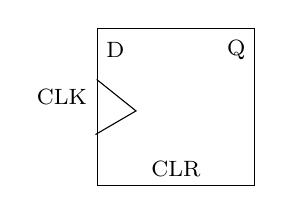
\begin{tikzpicture}
  [every node/.style={font=\footnotesize},
  ff/.style={minimum width=2cm,minimum height=2cm,draw}]
  \def\d{8}
  \node[ff] (DFF) {};
  \node[right] at (DFF.north west)[yshift=-\d] {D};
  \path[draw] (DFF.west)+(0,.35) node[below left] {CLK} -- +(.5,-.05) -- +(-.015,-.35);
  
  \node[left] at (DFF.north east)[yshift=-\d] {Q};
  \node[above] at (DFF.south) {CLR};
\end{tikzpicture}
\caption{Flip-flop tipo D com entrada {\em CLEAR}.}
\label{fig:dff}
\end{figure}

\begin{center}
\begin{tikztimingtable}[timing/slope=0,xscale=2,
  yscale=1.5,semithick]
  Clock & 12{C} \\
  CLR &  5.75L .5H 5.75L\\
  Entrada D &2H 2L 4H 4L\\
  Saída Q &   \\
  \extracode
  \begin{pgfonlayer}{background}
    \begin{scope}[gray ,semitransparent,dashed,semithick]
      \foreach \x in {1,...,12}
      \draw (\x,1) -- (\x,-8);
    \end{scope}
  \end{pgfonlayer}
\end{tikztimingtable}
\end{center}

\begin{solution}
\begin{center}
\begin{tikztimingtable}[timing/slope=0,xscale=2,
  yscale=1.5,semithick]
  Clock & 12{C} \\
  CLR &  5.75L .5H 5.75L\\
  Entrada D &2H 2L 4H 4L\\
  Saída Q &  1L 2H 2L .75H 1.25L 2H 3L\\
  \extracode
  \begin{pgfonlayer}{background}
    \begin{scope}[gray ,semitransparent,dashed,semithick]
      \foreach \x in {1,...,12}
      \draw (\x,1) -- (\x,-8);
    \end{scope}
  \end{pgfonlayer}
\end{tikztimingtable}
\end{center}
\end{solution}

}

\def\DTFF{ \question[1,5]~A Figura~\ref{fig:dtff} mostra as formas de
  onda aplicadas a um flip-flop tipo D disparado por borda de
  descida. Este mesmo flip-flop pode ser comutado para funcionar como
  um flip-flop do tipo T. Desenhe a forma de onda de saída para o
  flip-flop atuando como tipo D ($Q_D$) e tipo T ($Q_T$).


\begin{figure}
\begin{center}
\begin{tikztimingtable}[timing/slope=0,xscale=2,
  yscale=1.5,semithick]
  Clock & 9{C} \\
  Entrada D & 1.5L 2H 1L 1H .25L 1.8H 1.4L\\
  Saída $Q_D$ &   \\
  Saída $Q_T$ &   \\
  \extracode
  \begin{pgfonlayer}{background}
    \begin{scope}[gray ,semitransparent,dashed,semithick]
      \foreach \x in {1,...,9}
      \draw (\x,1) -- (\x,-8);
    \end{scope}
  \end{pgfonlayer}
\end{tikztimingtable}
\end{center}
\caption{Sinais de entrada para um flip-flop do tipo D, que pode ser
  comutado para o tipo T.}
\label{fig:dtff}
\end{figure}

}

\def\COUNTER{

\question[2]

\begin{parts}

\part

Projete um contador ASSÍNCRONO que conte de 0 a 9 utilizando FF
ativados na borda de descida.

\part
Qual o tempo mínimo que deve ser esperado para fazer a leitura das
saídas após a borda de descida do clock?  

\noindent Obs: Considere que cada FF demore 200ns para
atualizar a saída após a borda de descida do clock

\end{parts}

}